\section*{Introduction}
The goal of this project is to optimize an algorithm by parallelization, utilizing the \texttt{C++} programming language in conjunction with various APIs and libraries, leading to distinct solutions, each with their advantages and disadvantages.
\par The algorithm computes a square matrix by following a Wavefront pattern across its upper diagonal. The process is as follows: given an upper-triangular square matrix \texttt{mtx} of size $n \times n$, only the elements on the main diagonal are known initially:
\begin{equation}
    \forall i \in [0, n - 1].mtx[i][i] = (i+1)/n  
\end{equation}
For each of the upper diagonals, the elements are computed as:
\begin{equation}
    \forall i \in [0, n - 1]. \forall j \in [i + 1, n - 1]. mtx[i][j] = \sqrt[3]{\sum_{k = 0}^{j - 1}mtx[i][k] * mtx[j][k + 1]}
\end{equation}
The element is obtained as the dot product between the row vector at index \textit{i} and the column vector at index \textit{j}, containing the elements prior to the one being computed. This means that to compute an element on the $\textit{z}^{th}$ diagonal, the elements of the previous diagonal must already be completed. In contrast, elements within the same diagonal can be computed independently of each other.

\begin{figure}[h]
    \centering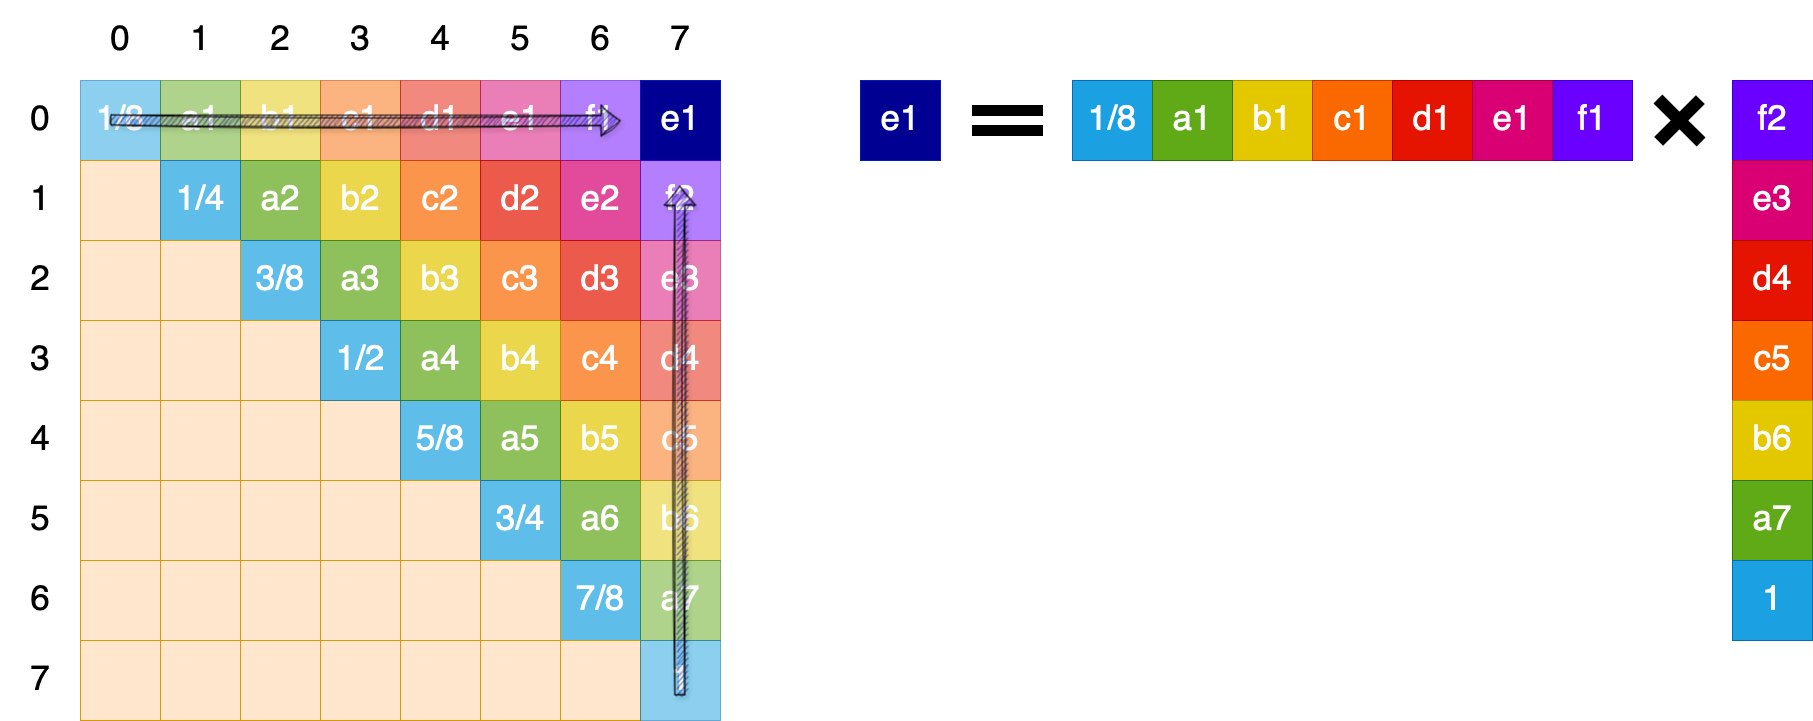
\includegraphics[scale=0.20]{img/Introduction/WaveFrontExample.png}
    
    \caption{Example of a 8x8 Matrix generated using the Wavefront Computation.}
\end{figure}
